% Template for Cogsci submission with R Markdown

% Stuff changed from original Markdown PLOS Template
\documentclass[10pt, letterpaper]{article}

\usepackage{cogsci}
\usepackage{pslatex}
\usepackage{float}
\usepackage{caption}

% amsmath package, useful for mathematical formulas
\usepackage{amsmath}

% amssymb package, useful for mathematical symbols
\usepackage{amssymb}

% hyperref package, useful for hyperlinks
\usepackage{hyperref}

% graphicx package, useful for including eps and pdf graphics
% include graphics with the command \includegraphics
\usepackage{graphicx}

% Sweave(-like)
\usepackage{fancyvrb}
\DefineVerbatimEnvironment{Sinput}{Verbatim}{fontshape=sl}
\DefineVerbatimEnvironment{Soutput}{Verbatim}{}
\DefineVerbatimEnvironment{Scode}{Verbatim}{fontshape=sl}
\newenvironment{Schunk}{}{}
\DefineVerbatimEnvironment{Code}{Verbatim}{}
\DefineVerbatimEnvironment{CodeInput}{Verbatim}{fontshape=sl}
\DefineVerbatimEnvironment{CodeOutput}{Verbatim}{}
\newenvironment{CodeChunk}{}{}

% cite package, to clean up citations in the main text. Do not remove.
\usepackage{cite}

\usepackage{color}

% Use doublespacing - comment out for single spacing
%\usepackage{setspace}
%\doublespacing


% % Text layout
% \topmargin 0.0cm
% \oddsidemargin 0.5cm
% \evensidemargin 0.5cm
% \textwidth 16cm
% \textheight 21cm

\title{From \emph{uh-oh} to \emph{tomorrow}\\Predicting age of acquisition for
early words across languages}


\author{{\large \bf Mika Braginsky} \\ \texttt{mikabr@stanford.edu} \\ Department of Psychology \\ Stanford University \And {\large \bf Daniel Yurovsky} \\ \texttt{yurovsky@stanford.edu} \\ Department of Psychology \\ Stanford University \And {\large \bf Virginia A. Marchman} \\ \texttt{marchman@stanford.edu} \\ Department of Psychology \\ Stanford University \And {\large \bf Michael C. Frank} \\ \texttt{mcfrank@stanford.edu} \\ Department of Psychology \\ Stanford University}

\begin{document}

\maketitle

\begin{abstract}
\emph{{[}TODO: abstract{]}}

\textbf{Keywords:}
language acquisition; word learning; development
\end{abstract}

\section{Introduction}\label{introduction}

One of the central problems facing a child acquiring their first
language is to learn word meanings. Learners must integrate multiple
information sources to figure out how to map the wordforms they hear
onto representations of their meanings. Across many labratory
experiments and small-scale models, a number of strategies have emerged
as plausible components of word learning, including tracking
co-occurence statistics between words and referents to deduce word
meaning across situations; attending to social cues like pointing and
eye gaze to direct hypothesis search; relying on certain biases, such as
priviledging basic level category labels, to constrain inference;
drawing on knowledge of relations between words to use known meanings to
learn new ones; and so on.

Each of these abilities has been reliably demonstrated in the
constrained learning contexts of the laboratory, indicating that they
could be used for word learning. But it is less clear to what extent
children actually employ them in the natural word learning environment
and how they interact to create the longer-term dynamics of vocabulary
acquisition. How do various word learning mechanisms differ in their
relative contributions, and how does that change over the course of
development?

One way to address these questions is to use naturalistic large-scale
vocabulary development data to examine the contribution of various
theoretically-relevant factors to vocabulary growth. We can look across
children to determine how easy or hard various words are to learn, and
then examine the relationship between words' difficulties and various
word properties that relate to proposed word learning mechanisms.
Foundational work using such an approach has revealed that in English,
within lexical category, words that are more frequent in speech to
children are likely to be learned earlier (J. C. Goodman, Dale, \& Li,
2008; B. C. Roy, Frank, \& Roy, 2009). Further studies have delved into
the relevance of semantic networks (Hills, Maouene, Maouene, Sheya, \&
Smith, 2009), neighborhood density (Stokes, 2010), iconocity (Perry,
Perlman, \& Lupyan, 2015), and linguistic distinctiveness (B. C. Roy,
Frank, DeCamp, Miller, \& Roy, 2015) to vocabulary construction.

However, the previous studies use different datasets, focus on different
predictors, and for the most part only analyze English data. It is thus
impossible to compare the relative importance of the many relevant
factors and to draw robust conclusions. To remedy this issue, we present
analyses based on data from Wordbank (wordbank.stanford.edu), an open
repository of language development data (Frank, Braginsky, Yurovsky, \&
Marchman, in press). By aggregating administrations of the
MacArthur-Bates Communicative Development Inventory (CDI; Fenson, 2007),
a family of parent-report vocabulary checklists, Wordbank provides
large-scale vocabulary data that we use to conduct analyses over
development and across languages.

We integrate Wordbank data with characterizations of the word learning
environment from the CHILDES database (MacWhinney, 2000) and elsewhere,
a multiple data source approach pioneered by J. C. Goodman et al.
(2008). Building on their work, we want to move beyond frequency to
examine a variety of information sources. We specifically follow B. C.
Roy et al. (2015) in predicting age of acquisition (AoA) as a function
of several different environment predictors. In analyzing a high-density
longitudinal corpus for a single English-acquiring child, Roy et al
found that frequency, number of characters, and mean length of
utterances were predictive of the age of a word's first production. Due
to the nature of the data, this analysis was limited to one language (in
fact to one subject) and could only test production, distancing the
connection between properties of the input and the child's emerging
understanding of words.

Our approach provides a complimentary analysis by using CDI
comprehension data to look at earliest words, across languages. We
estimate the age of acquisition for around 400 words in each of 7
languages. We also estimate each words' frequency and mean length of
utterances (MLU) in which it appears, as well as obtaining ratings of
each words' concreteness, valence, arousal, and relevance to babies from
previously collected norms. We then predict words' AoA from all of these
properties, and assess the relative contributions of each factor, along
with the interaction of predictors with the lexical category and their
changes over development. Each of these analyses has the potential to
provide leverage on long-standing theoretical questions.

A first theoretical question of interest is which lexical categories are
most influenced by input-related factors like frequency and utterance
length compared with conceptual factors like concreteness or valence.
For example, ``division of dominance'' theory suggests that nouns might
be more sensitive to cognitive factors while predicates and closed-class
words might be more sensitive to linguistic factors (Gentner \&
Boroditsky, 2001). On the other hand, on syntactic bootstrapping
theories, nouns are argued to be learned via frequent co-occurrence
(operationalized by frequency) while verbs might be more sensitive to
syntactic factors (operationalized here by utterance length) (Gleitman,
1990), and neither would be particularly sensitive to conceptual
complexity (Snedeker, Geren, \& Shafto, 2007).

A second question of interest is the variability across languages in the
relative importance of predictors. For example, are there differences in
the importance of syntactic factors in morphologically more complex
languages like Russian and Turkish, compared with simpler ones like
English? Differences of this type might be revealing of the degree to
which learners face different challenges in different language
environments. Or consistency may suggest the operation of similar
learning mechanisms and strategies that are not as dependent on the
complexities of phonology, morphology, and syntax in a particular
language.

Overall, by incorporating a variety of theoretically-important factors,
as well as basing our analysis on a large samples of words and children
and building towards more cross-linguistic coverage, our study presents
a more thorough investigatation of the question of what properties
determine words' learnability.

\section{Data}\label{data}

We use Wordbank (wordbank.stanford.edu), an open database of
developmental vocabulary data, to estimate the age of acquisition for
words across 7 languages: English, Italian, Norwegian, Russian, Spanish,
Swedish, Turkish. We then ask what factors are most important for
predicting this age of acquisition.

\subsection{Estimating Age of
Acquisition}\label{estimating-age-of-acquisition}

To estimate the age at which words are acquired, we took vocabulary data
collected using the MacArthur-Bates Communicative Development Inventory,
a family of parent-report checklists, specifically the Words \& Gestures
(infant) form for 8- to 18-month-olds. When filling out a CDI a form,
parents are asked to indicate whether their child understands and/or
says each of around 400 words. From these data, for each word on the
CDI, we computed the proportion of children at each age that are
reported to understand the word. We then fit a logistic curve to these
proportions using a robust generalized linear model (using the
\texttt{robustbase} package in \texttt{R}) and determine when the curve
crosses 0.5, i.e.~at what age at least 50\% of children are reported to
understand the word. Following J. C. Goodman et al. (2008), we take this
point to be each word's age of acquisition.

\begin{table}[t]
\centering
\begin{tabular}{lrrr}
  \hline
Language & CDI Items & CDI Admins & CHILDES Words \\ 
  \hline
English & 386 & 2,452 & 7,858,051 \\ 
  Italian & 351 & 648 & 328,168 \\ 
  Norwegian & 338 & 3,021 & 204,406 \\ 
  Russian & 337 & 768 & 32,398 \\ 
  Spanish & 333 & 778 & 1,458,327 \\ 
  Swedish & 311 & 467 & 698,515 \\ 
  Turkish & 327 & 1,115 & 44,347 \\ 
   \hline
\end{tabular}
\caption{Dataset statistics} 
\end{table}

\begin{table}[!hb]
\centering
\begin{tabular}{ll}
  \hline
Measure & Words \\ 
  \hline
aoa & mommy, bottle, peekaboo \\ 
   & babysitter, teacher, naughty \\ 
  frequency & living room, cockadoodledoo, grrr \\ 
   & you, it, that \\ 
  babiness & donkey, penny, jeans \\ 
   & baby, bib, bottle \\ 
  concreteness & how, now, that \\ 
   & apple, ball, banana \\ 
  mlu & cockadoodledoo, peekaboo, uh oh \\ 
   & babysitter, when (question), day \\ 
  arousal & shh, asleep, blanket \\ 
   & naughty, money, scared \\ 
  valence & sick, owie, ouch \\ 
   & happy, hug, love \\ 
  num\_characters & i, in, it \\ 
   & cockadoodledoo, refrigerator, living room \\ 
   \hline
\end{tabular}
\caption{Examples of words with the lowest and highest values for age of acquisition and each predictor.} 
\label{tab:mytable}
\end{table}

\begin{CodeChunk}
\begin{figure*}[!h]

{\centering 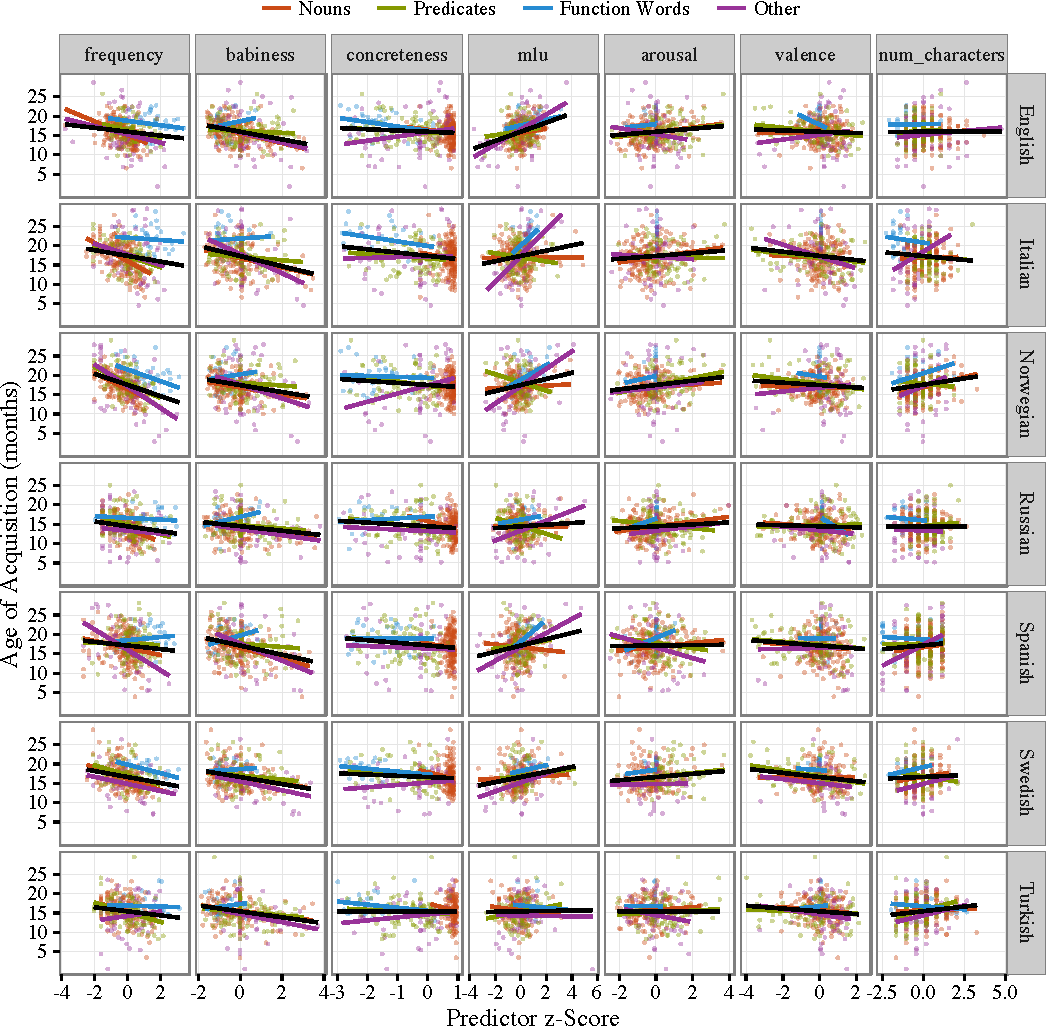
\includegraphics{figs/data-1} 

}

\caption[Relationship between predictors and AoA for each lexical category in each language]{Relationship between predictors and AoA for each lexical category in each language.}\label{fig:data}
\end{figure*}
\end{CodeChunk}

\begin{CodeChunk}
\begin{figure*}[tb]

{\centering 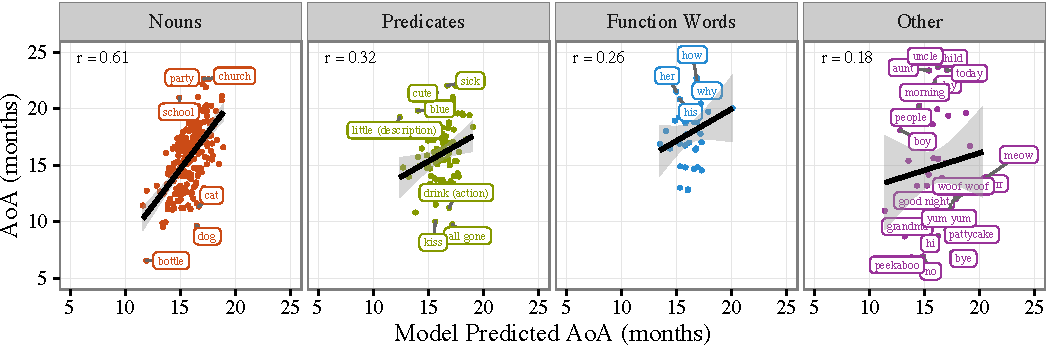
\includegraphics{figs/fit-1} 

}

\caption[English model fit]{English model fit.}\label{fig:fit}
\end{figure*}
\end{CodeChunk}

\begin{CodeChunk}
\begin{figure}[!hb]

{\centering 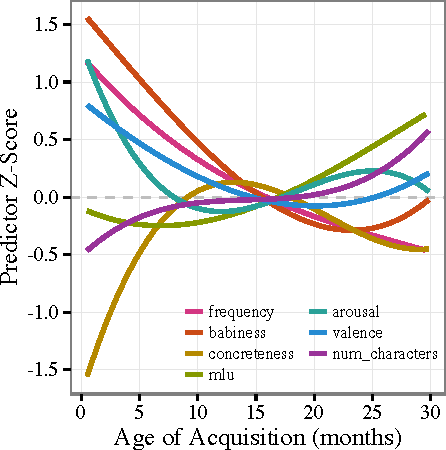
\includegraphics{figs/devo-1} 

}

\caption[Predictor values over development]{Predictor values over development.}\label{fig:devo}
\end{figure}
\end{CodeChunk}

\begin{CodeChunk}
\begin{figure*}[tb]

{\centering 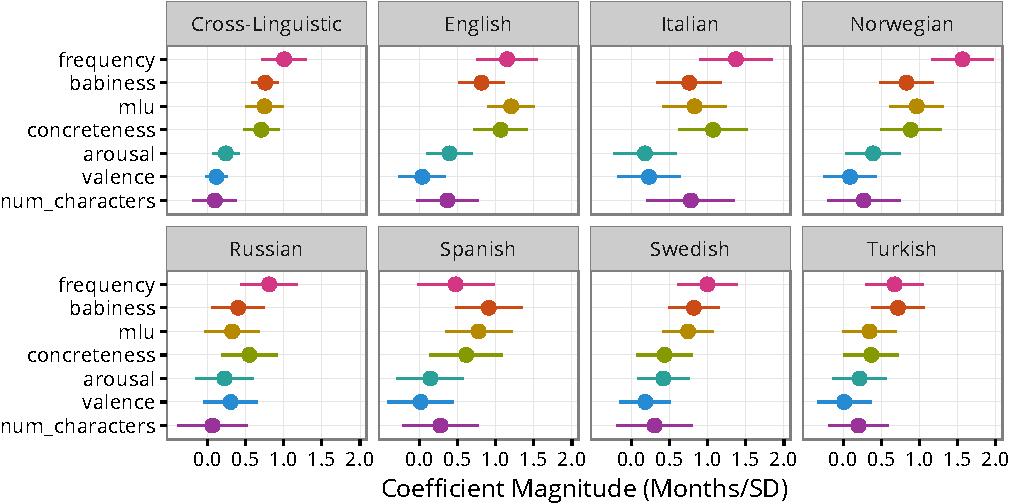
\includegraphics{figs/coefs-1} 

}

\caption[Magnitudes of predictor coefficients]{Magnitudes of predictor coefficients.}\label{fig:coefs}
\end{figure*}
\end{CodeChunk}

\begin{CodeChunk}
\begin{figure*}[tb]

{\centering 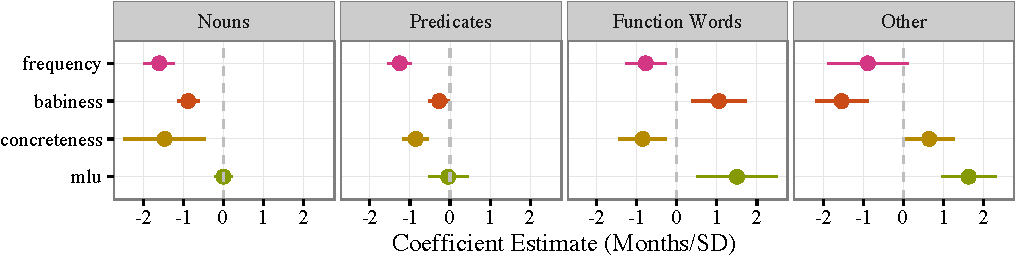
\includegraphics{figs/coefs_lexcat-1} 

}

\caption[Magnitudes of predictor coefficients by lexical category]{Magnitudes of predictor coefficients by lexical category.}\label{fig:coefs_lexcat}
\end{figure*}
\end{CodeChunk}

\subsection{Predictors}\label{predictors}

Each of our predictors are derived from independent resources. For each
word that appears on the CDI Word \& Gestures form in each of our 7
languages, we obtained an estimate of its frequency in child-directed
speech, the mean utterance length (MLU) of sentences in which if appears
in child-directed speech, its length in characters, and ratings of its
concreteness, valence, arousal, and relevance to babies. Examples of
each of these predictors for English are shown in Table
\ref{tab:extremes}.

While frequency and MLU are measured relative to the word's language,
since the conceptual ratings were collected only in English, we mapped
all the words onto translation equivalents across CDI forms, allowing us
to use the ratings for English words cross-linguistically. While
imperfect, this method allows us to examine languages for which limited
resources exist. Translation equivalents are available in the wordbank
database using the \texttt{wordbankr} package (Frank et al., in press).

Items such as \emph{child's own name} were excluded in all languages.
Each predictor was also centered and scaled so that all predictors would
have comparable units. Lexical category was determined on the basis of
the conceptual categories presented on the CDI form (e.g., ``Animals''),
such that Nouns contains common nouns, Predicates contains verbs and
adjectives, Function Words contains closed-class words, and Other
contains the remaining items (following Bates et al., 1994).

\subsubsection{Frequency}\label{frequency}

For each language, we estimated word frequency from unigram count in all
corpora in the CHILDES database for that language, normalized to the
length of the corpus. Each word's count includes the counts of words
that share the same stem (so that \emph{dogs} counts as \emph{dog}) or
are synonymous (so that \emph{father} counts as \emph{daddy}). For
polysemous word pairs, such as \emph{orange} as in color and
\emph{orange} as in fruit, each occurence of \emph{orange} in the corpus
counts for both. Finally, each word's frequency estimate is taken as the
log of its count.

\subsubsection{MLU}\label{mlu}

For each language, we estimated each word's MLU by calculating the mean
number of words in the sentences in which that word appears in all
corpora in the CHILDES database for that language. Words that only occur
in one sentence were excluded.

\subsubsection{Length}\label{length}

We computed the number of characters in each word in each language,
which is known to be highly correlated with number of phonemes and
syllables.

\subsubsection{Concreteness}\label{concreteness}

We used previously collected norms for concreteness (Brysbaert,
Warriner, \& Kuperman, 2014), which were gathered by asking adult
participants to rate how concrete the meaning of each word is by using a
5-point scale from abstract to concrete. For the 120 CDI words that
weren't part of the collected norms (mostly animal sounds such as
\emph{baa baa}), we imputed a conreteness rating from the mean of all
CDI words' concreteness rating.

\subsubsection{Valence and Arousal}\label{valence-and-arousal}

We also used previously collected norms for valence and arousal
(Warriner, Kuperman, \& Brysbaert, 2013), for which adult participants
are asked to rate words on a 1-9 happy-unhappy scale (valence) and 1-9
excited-calm scale (arousal). For the 119 CDI words that weren't part of
the collected norms (mostly function words such as \emph{her}), we
imputed ratings from the mean of all CDI words' ratings.

\subsubsection{Babiness}\label{babiness}

Lastly, we used previously collected norms of ``babiness'', a measure of
association with infancy (Perry et al., 2015) for which adult
participants are asked to judge how relevant to babies a word is.

\section{Analysis}\label{analysis}

An overview of our entire dataset can be seen in Figure \ref{fig:data},
which shows each word's estimated age of acquisition against its
predictor values, separated by language and lexical category. We present
three analyses of these data: 1) how predictor values change for words
learned earlier and later, 2) their relative contributions to predicting
AoA, and 3) their interaction with lexical category.

\subsection{Developmental Trajectory}\label{developmental-trajectory}

To assess developmental trends, we examine how the values of each
predictor change as a function of estimated AoA. Figure \ref{fig:devo}
shows these trajectories, with a cubic curve smoothing over all words.
Words that are learned earlier are more frequent, higher in babiness,
and appear in shorter sentences. Concreteness exhibits a U-shaped
trajectory, with the earliest learned words actually being relatively
abstract, such as many social routines and animal sounds.

\subsection{Predicting AoA}\label{predicting-aoa}

We fit a linear regression for each language's data, as well as a linear
mixed-effects model with language as a random effect for all the data
pooled. For illustrative purposes, Figure \ref{fig:fit} compares the
predictions of the model to AoA estimates, for only English data, with
outliers labelled.

Figure \ref{fig:coefs} shows the magnitude and direction of the
coefficient for each predictor in each language and
cross-linguistically. We find that frequency, babiness, concreteness,
and MLU are relatively stronger predictors of age of acquisition, across
languages and in the cross-linguistic model. Overall there's
considerable consistency in how the predictors pattern in various
languages, although with interesting differences: for example, MLU in
English appears to be unusually strong, while frequency in Spanish look
unusually weak. There is also variability in the overall fit of the
models to the data, with some languages, such as Norwegian, having
relatively more of the variance explained than others, such as Turkish.

\subsection{Lexical Category}\label{lexical-category}

Previous work gives reason to believe that predictors' relationship with
age of acquisition differs among various lexical categories (J. C.
Goodman et al., 2008). To investigate these effects, we break down our
data by lexical category and fit separate cross-linguistic linear
mixed-effects models for each one. Figure \ref{fig:coefs_lexcat} shows
the magnitudes and directions of the resulting coefficients, leaving off
the less strong predictors. We find that frequency matters most for
Nouns and comparatively little for Function Words, while MLU is
irrelevant for both Nouns and Predicates, but highly informative for
Function Words and Other items.

\emph{{[}TODO: mention predictors' correlations to each other{]}}

\emph{{[}TODO: mention that predictors have different variabilities,
that probably matters{]}}

\emph{{[}TODO: emphasize the sketchiness of using ratings
cross-linguistically{]}}

\section{Discussion}\label{discussion}

What makes words easier or harder for young children to learn? Previous
experimental work has largely addressed this question using small-scale
experiments. While such experiments can identify sources of variation,
they typically do not allow for different sources to be compared in
detail. In contrast, observational studies allow the effects of
individual factors (with frequency being the most common) to be measured
across ages and lexical categories (e.g., J. C. Goodman et al., 2008).
Scale comes at a cost in terms of detail, however: Both the predictors
and outcome data available have been quite limited.

By including 7 languages and as many predictors, our current work
expands the scope of previous observational studies of age of
acquisition. Our data show a number of patterns that confirm and expand
previous reports. First, predictors differed in importance across even
very early development. For example, certain concepts that were more
strongly associated with babies appeared to be learned early for
children across languages (Tardif et al., 2008). Second, we found
general consistency in predictor coefficients across languages (even as
overall model fit varied, at least in part due to the amount and quality
of data for different languages). This consistency supports the idea
that differences in culture or language structure do not lead to
fundamentally different acquisition strategies.

Finally, different predictors appeared more important across lexical
categories. Frequent, concrete nouns were learned earlier, consistent
with theories that emphasize the importance of early referential speech
(e.g., Baldwin, 1995). But for predicates, concreteness was somewhat
less important, and for function words, MLU was most predictive. Overall
thse findings are consistent with theories that emphasize the role of
linguistic structure over conceptual complexity in the acquisition of
other lexical categories beyond nouns (Gentner \& Boroditsky, 2001,
Snedeker et al. (2007)).

Despite its larger scope, our work still shares a number of important
limitations with previous studies. First and foremost, our approach is
to predict one set of individuals with data about the experience of a
completely different set and ratings of concepts gathered from yet
others. In contrast to dense-data approaches (B. C. Roy et al., 2015),
this approach fundamentally limits the amount of variability we will be
able to capture. In addition, the granularity of the predictors that can
be extracted from corpus data and applied to every word is necessarily
quite coarse. Ideally, predictors could be targeted more specifically at
particular theoretical constructs of interest (for example, the patterns
of use for particular predicates).

Perhaps the most important theoretical challenge in the study of early
language is hwo to connect between the scale of an individual
observation or experiment and the broader patterns of acquisition that
we observe in large datasets. We have strong theories of how individual
learning situations proceed (M. C. Frank, Goodman, \& Tenenbaum, 2009,
McMurray, Horst, \& Samuelson (2012)). We may not yet be able to discern
the unambiguous signatures of these theories in the aggregate data we
have available. But we believe that searching for these signatures at
scale is a critical step in making progress on understanding language
learning.

\section{Acknowledgements}\label{acknowledgements}

Thanks to the MacArthur-Bates CDI Advisory Board. This work supported by
NSF BCS \#1528526.

\section{References}\label{references}

\setlength{\parindent}{-0.1in} \setlength{\leftskip}{0.125in} \noindent

Baldwin, D. A. (1995). Understanding the link between joint attention
and language. \emph{Joint Attention: Its Origins and Role in
Development}, 131--158.

Bates, E., Marchman, V., Thal, D., Fenson, L., Dale, P., Reznick, J. S.,
\ldots{} Hartung, J. (1994). Developmental and stylistic variation in
the composition of early vocabulary. \emph{Journal of Child Language},
\emph{21}(01), 85--123.

Brysbaert, M., Warriner, A. B., \& Kuperman, V. (2014). Concreteness
ratings for 40 thousand generally known English word lemmas.
\emph{Behavior Research Methods}, \emph{46}(3), 904--911.

Fenson, L. (2007). \emph{MacArthur-Bates Communicative Development
Inventories: User's guide and technical manual}. Paul H. Brookes
Publishing Company.

Frank, M. C., Braginsky, M., Yurovsky, D., \& Marchman, V. A. (in
press). Wordbank: An open repository for developmental vocabulary data.
\emph{Journal of Child Language}.

Frank, M. C., Goodman, N. D., \& Tenenbaum, J. B. (2009). Using
speakers' referential intentions to model early cross-situational word
learning. \emph{Psychological Science}, \emph{20}, 578--585.

Gentner, Dedre, \& Boroditsky, L. (2001). Individuation, relativity, and
early word learning. \emph{Language Acquisition and Conceptual
Development}, \emph{3}, 215.

Gleitman, L. (1990). The structural sources of verb meanings.
\emph{Language Acquisition}, \emph{1}(1), 3--55.

Goodman, J. C., Dale, P. S., \& Li, P. (2008). Does frequency count?
Parental input and the acquisition of vocabulary. \emph{Journal of Child
Language}, \emph{35}(3), 515.

Hills, T. T., Maouene, M., Maouene, J., Sheya, A., \& Smith, L. (2009).
Longitudinal analysis of early semantic networks: Preferential
attachment or preferential acquisition? \emph{Psychological Science},
\emph{20}(6), 729--739.

MacWhinney, B. (2000). \emph{The CHILDES project: The database} (Vol.
2). Psychology Press.

McMurray, B., Horst, J. S., \& Samuelson, L. K. (2012). Word learning
emerges from the interaction of online referent selection and slow
associative learning. \emph{Psychological Review}, \emph{119}(4), 831.

Perry, L. K., Perlman, M., \& Lupyan, G. (2015). Iconicity in English
and Spanish and its relation to lexical category and age of acquisition.
\emph{PloS One}, \emph{10}(9), e0137147.

Roy, B. C., Frank, M. C., \& Roy, D. (2009). Exploring word learning in
a high-density longitudinal corpus. \emph{Proceedings of the Cognitive
Science Society}.

Roy, B. C., Frank, M. C., DeCamp, P., Miller, M., \& Roy, D. (2015).
Predicting the birth of a spoken word. \emph{Proceedings of the National
Academy of Sciences}, \emph{112}(41), 12663--12668.

Snedeker, J., Geren, J., \& Shafto, C. L. (2007). Starting over
international adoption as a natural experiment in language development.
\emph{Psychological Science}, \emph{18}(1), 79--87.

Stokes, S. F. (2010). Neighborhood density and word frequency predict
vocabulary size in toddlers. \emph{Journal of Speech, Language, and
Hearing Research}, \emph{53}(3), 670--683.

Tardif, T., Fletcher, P., Liang, W., Zhang, Z., Kaciroti, N., \&
Marchman, V. A. (2008). Baby's first 10 words. \emph{Developmental
Psychology}, \emph{44}(4), 929.

Warriner, A. B., Kuperman, V., \& Brysbaert, M. (2013). Norms of
valence, arousal, and dominance for 13,915 English lemmas.
\emph{Behavior Research Methods}, \emph{45}(4), 1191--1207.

\end{document}
